\documentclass[12pt]{article}
\usepackage{float}
\usepackage[utf8]{inputenc}
\usepackage[T1]{fontenc}
\usepackage{outline}
\usepackage{pmgraph}
\usepackage[normalem]{ulem}
\usepackage{amsmath,mathdots}
\usepackage{amsfonts,amssymb,amsthm,yhmath}
\usepackage{fancyhdr}
\usepackage{graphicx}
\usepackage{multicol}
\usepackage{vmargin}
\usepackage{physics}
\usepackage{cancel}
\usepackage{multicol,multirow}
\usepackage{bm}
\usepackage{hyperref}
\usepackage[scaled]{helvet}
\usepackage{color}
\usepackage{siunitx}
\usepackage{array}
\usepackage{gensymb}
\usepackage{tabularx}
\usepackage{extarrows}
\usepackage{booktabs}
\usepackage{bbold, dsfont}
\usepackage{authblk}
\usepackage{subcaption}
\hypersetup{
    colorlinks=true,
    linkcolor=black,
    filecolor=magenta,
    urlcolor=blue,
}
\renewcommand{\Authand}{ y }
\renewcommand{\Affilfont}{\itshape\small}
%\usepackage{minted}


\title{Python Function of Runge Kutta Method}
\author{Merlyn JJG}

\begin{document}
\maketitle

\section{Four Order Runge Kutta Method }
\label{sec:rk4}

Runge–Kutta method is an effective and widely used, iterative method
for solving ordinary differential equations
\(\frac{dr(t)}{dt}=f(r,t)\). Runge–Kutta methods perform several
evaluation of the function \(f()\) around a point \((r(t_{n}),t_{n})\)
and then the point \(r(t_{n+1})\) is computed using a weighted average
of the derivatives \(f()\) values. The derivative function is
evaluated in approximated points that might be contained in the
original solution.

The Runge-Kutta of four order is defined using the following recursion
formula,
\begin{equation}
  \label{eq:RecursionFormulaeSolution}
  r_{n+1} = r_{n} + \frac{1}{6}(k_{1}+k_{2}+k_{3}+k_{4}),
\end{equation}
where the \(k's\) are the slopes values evaluated at the different
points, these given by the function \(f()\) evaluated as follow
\begin{subequations}
  \begin{equation}
    \label{eq:slope1}
    k_{1}= f(r_{0},t_{0}),
  \end{equation}
  \begin{equation}
    \label{eq:slope2}
    k_{2}= f(r_{0}+k_{1}\frac{h}{2},t_{0}+\frac{h}{2}),
  \end{equation}
  \begin{equation}
    \label{eq:slope3}
    k_{3}= f(r_{0}+k_{2}\frac{h}{2},t_{0}+\frac{h}{2}),
  \end{equation}
    \begin{equation}
    \label{eq:slope4}
    k_{4}= f(r_{0}+k_{3}h, t_{0}+h),
  \end{equation}
\end{subequations}
where \(k_{1}\) is the beginnig slope, \(k_{2},k_{3}\) two midpoint
slopes and the endpoint slope \(k_{4}\), as shown in the figure
\ref{fig:CurveSlopes}
\begin{figure}
  \centering
  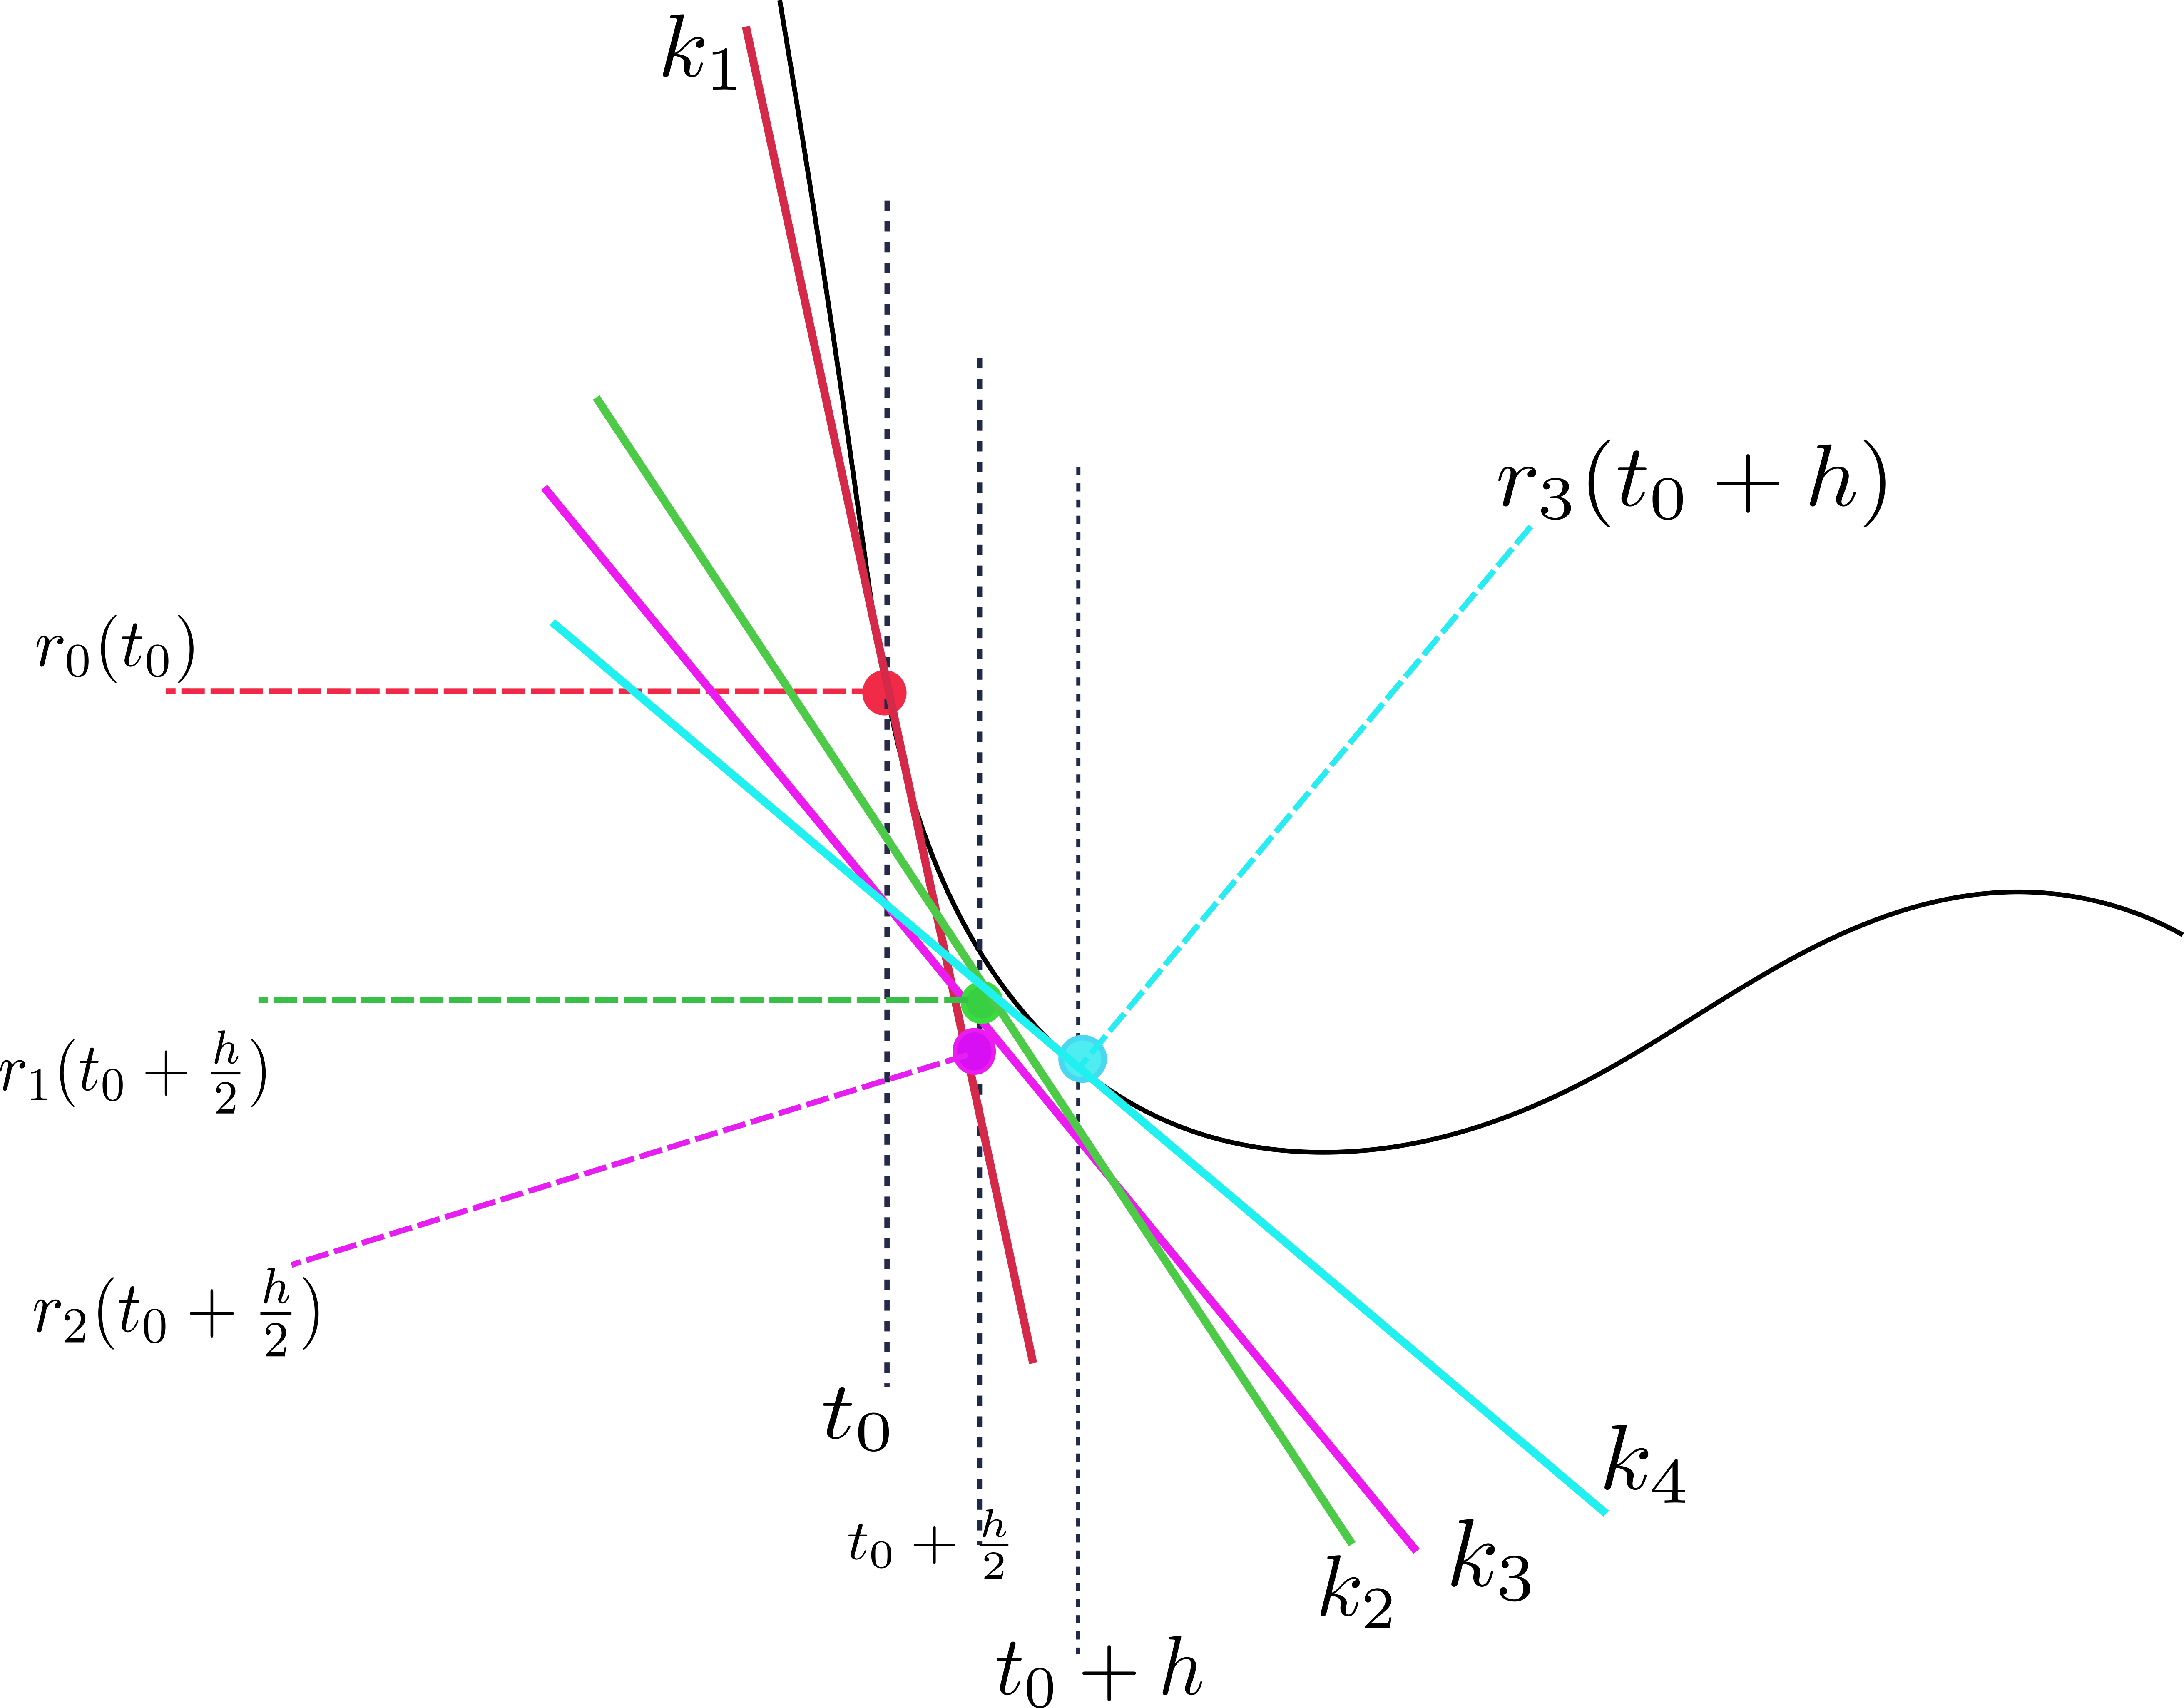
\includegraphics[width=0.7\textwidth]{CurveSlopes.png}
  \caption[Slopes]{Evaluation of the function $f()$ around the point $(r(t_{n}),t_{n})$
to obtain the slopes and perform the approximation.}
\label{fig:CurveSlopes}
\end{figure}

The generalization of to vectorial functions is straightfoward as well
as for second order differential equations.

The code solve the vectorial equation which can be written in a unique
function, but because of a matter of code clean up taste the first and
second order differential equations method applications are explicitly
given.

\subsection{Vectorial Differential Equation}
\label{sec:VectorialDE}

To clarify the usage of the method and so the functions
delivered in this work, the generalization can be explicitly
written as follows. Consider the the differential equation as,
\begin{equation}
  \label{eq:DiffEq}
  \frac{d\vec{r}(t)}{dt} = \vec{F}(\vec{r},t,parameters).
\end{equation}
where the function \(\vec{F}()\) contains the for example the partial
derivatives of \(\vec{r}\). The slopes of the method are vectorial
since are the function itself evaluated. Lorentz oscillator is the
chosen example to ilustrate this vectorial solution, shown at the end
of the file.

\section{First Order Differential Equation Function}
\label{sec:FODE}

Numerical integration within an interval of integration, suppose
\(t=(t_{0},t_{f})\) to get the solution of the differential equation,
\begin{equation}
  \label{eq:DiffEq}
  \frac{d\vec{r}(t)}{dt}=f(\vec{r},t,parameters).
\end{equation}
where parameters are parameters of the function. As theory of
differential equations tell us all the time, to find the solution of a
differential equation we need the initial conditions,
\((t_{0},\vec{r}_{0})\). The applying the RK method one finds the
slopes and the approximated solution as stated in the equations
(\eqref{eq:slope1}-\eqref{eq:slope4}) and
\eqref{eq:RecursionFormulaeSolution}.

\section{Second Order Differential Equation Function}
\label{sec:SecondODEFunction}

The ordinary second order differential equations have the following form
\begin{equation}
  \label{eq:SecondODE}
  \frac{d^{2}\vec{r}}{dt^{2}} = \vec{F}(\vec{r},\dot{\vec{r}},t,parameters),
\end{equation}
and are similarly solved as the first order differential equations but
solving both the first derivative and the the function desired, at
once. Because of the number of terms in the second order 
differential equation case grows, I avoid writting the vector form of the
equations.

The approximated first derivative is recursively obtained as
\begin{equation}
  \label{eq:RecursionFirstDerivative}
  \dot{r}_{n+1} = \dot{r}_{n} + \frac{1}{6}(k_{1}+k_{2}+k_{3}+k_{4}),
\end{equation}
and is used to obtain the approximated solution of the function as in
\eqref{eq:RecursionFormulaeSolution}. In
\eqref{eq:RecursionFirstDerivative} the \(k's\) are the second
derivatives, the slopes of the first derivative function curve at
different points around one given by the function \(\vec{F}()\)
evaluated as,
\begin{equation}
  \label{eq:First1}
  k_{1}= F(r_{0},\dot{r}_{0},t_{0}),
\end{equation}
used to obtain the first derivative and solution stepping halfway
through the time step,
\begin{equation}
  \label{eq:velocity1}
  \dot{r}1 = \dot{r}_{0} + k_{1}*h/2,
\end{equation}
\begin{equation}
  \label{eq:Sol_1}
  r1 = r_{0} + h*\frac{(\dot{r}_{0}+\dot{r}1)}{2},
\end{equation}
and similarly the other slopes and approximations,
\begin{equation}
  \label{eq:slope2}
  k_{2}= F(r1, \dot{r}1, t_{0}+\frac{h}{2}),
\end{equation}
\begin{equation}
  \label{eq:velocity2}
  \dot{r}2 = \dot{r}_{0} + k_{2}*h/2,
\end{equation}
\begin{equation}
  \label{eq:Sol_2}
  r2 = r_{0} + h*\frac{(\dot{r}_{0}+\dot{r}2)}{2},
\end{equation}
\begin{equation}
  \label{eq:slope3}
  k_{3}= F(r2, \dot{r}2, t_{0}+\frac{h}{2}),
\end{equation}
\begin{equation}
  \label{eq:velocity2}
  \dot{r}3 = \dot{r}_{0} + k_{3}*h/2,
\end{equation}
\begin{equation}
  \label{eq:Sol_2}
  r3 = r_{0} + h*\frac{(\dot{r}_{0}+\dot{r}3)}{2},
\end{equation}
\begin{equation}
  \label{eq:slope4}
  k_{4}= F(r3,\dot{r}3,t_{0}+h),
\end{equation}
so, the approximated first derivative and solution are given by the
average of their corresponding slopes,
\begin{equation}
  \dot{r}_{n+1} = \dot{r}_{n} + \frac{1}{6}(k_{1}+k_{2}+k_{3}+k_{4}), \tag{\ref{eq:RecursionFirstDerivative}}
\end{equation}
and
\begin{equation}
   \label{eq:SODE_Sol}
  r_{n+1} = r_{n} + \frac{1}{6}(\dot{r}1+\dot{r}2+\dot{r}3+\dot{r}_{n+1}).
\end{equation}



\end{document}
